\chapter{色谱法}\label{ch:b2:chromatography}

一滴能量饮料经稀释、过滤后，注入一根不比笔长的钢管中，
管内填充着直径仅几微米的硅胶颗粒。几分钟后，检测器
绘出一张带有几个峰的色谱图，由其中一个峰的面积，实验室报告该罐
饮料所含咖啡因的量，精确到百分之几。色谱法使混合物的各组分
以不同速率穿过色谱柱而得以分离；本章将说明它们为何以不同速率运动，
各峰为何具有这样的宽度、如何分开相邻的两种组分，以及如何把一个峰
换算为定量结果。

\begin{omfigure}
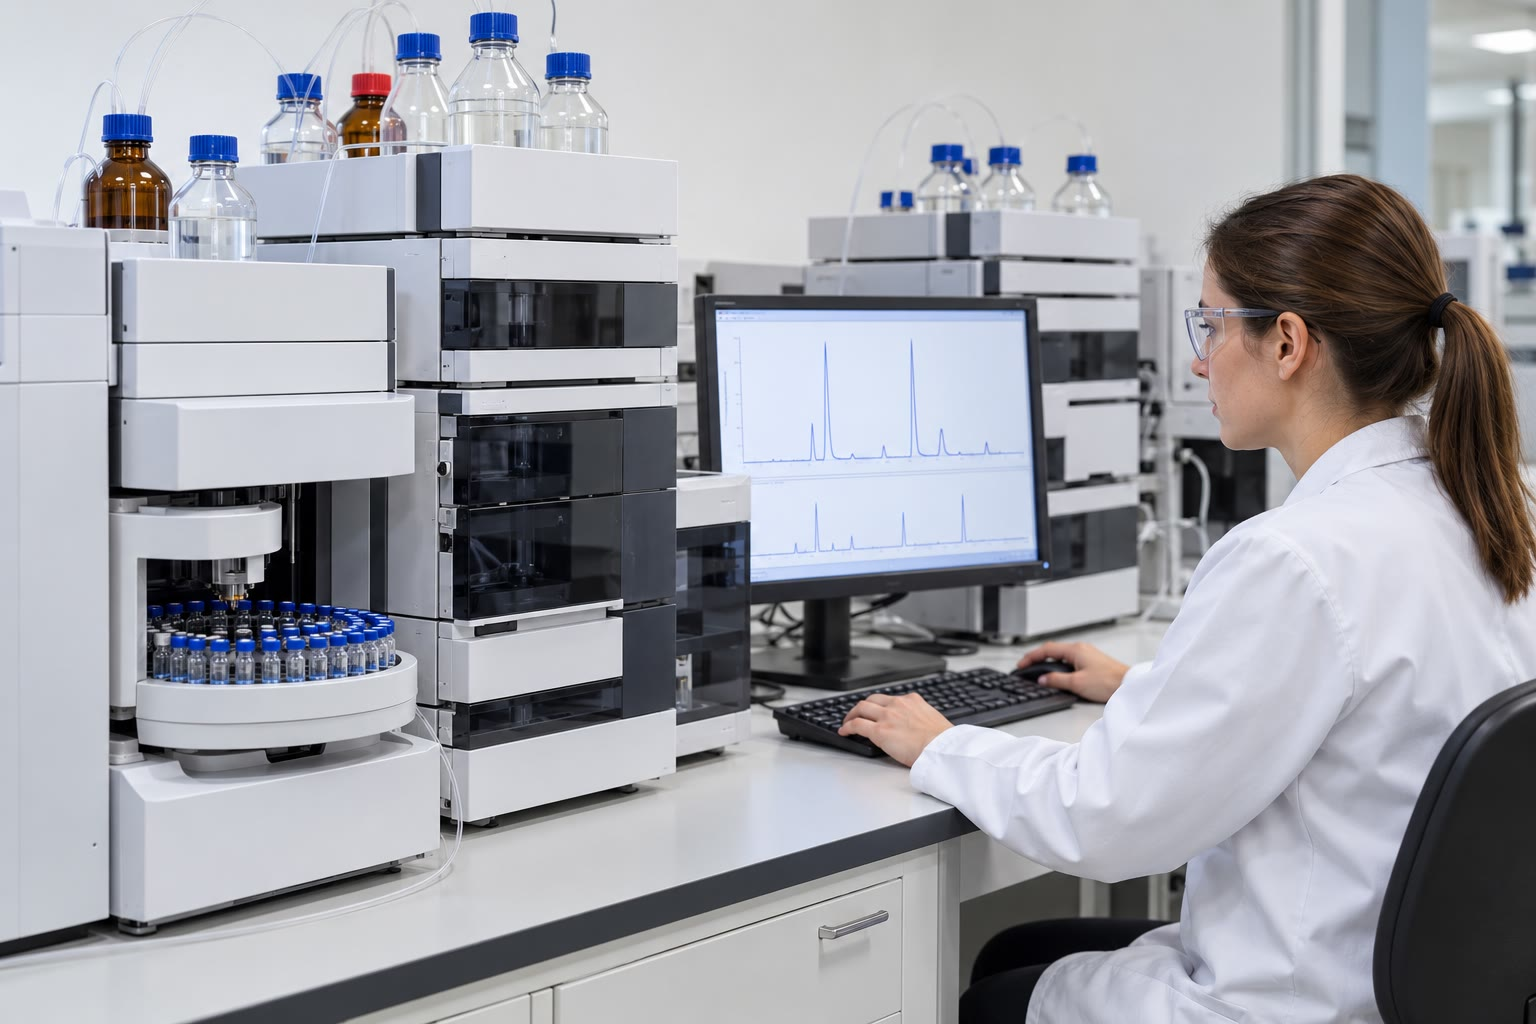
\includegraphics[width=0.58\linewidth]{images/book3/ai/b2-31-analytical-lab.jpg}

{\small 分析实验室：配有溶剂瓶的液相色谱仪及自动进样器，
样品瓶托盘；色谱图显示在屏幕上（示意图）。}
\end{omfigure}

\begin{recall}
第 1 册：纸色谱与薄层色谱法、色谱图、洗脱剂。本科一年级分册：
分配系数、液–液萃取，以及薄层板上的比移值 $R_f$。
\Cref{ch:b2:liquid-vapour-diagrams}：蒸馏塔的理论塔板。
\end{recall}

\section{原理}

\begin{definition}[色谱法]\label{def:b2:chromatography:principle}
\emph{色谱法}\index{色谱法}通过使混合物的各组分在
固定于色谱柱中或平板上的\emph{固定相}\index{固定相}与
\emph{流动相}\index{流动相}之间进行分配，流动相为流经固定相的气体或液体。
用流动相把各组分带过并带出色谱柱，称为\emph{洗脱}\index{洗脱}。
\end{definition}

分子只在流动相中运动；当它被固定相截留时，
便只能等待。它在行进途中要在两相之间切换数百万次，因此其平均速率
取决于它在两相中各自停留的时间比例，即取决于其分配平衡。

\begin{definition}[保留]\label{def:b2:chromatography:retention}
化合物的\emph{保留时间}\index{保留时间} $t_R$ 为从进样到
峰顶的时间；\emph{死时间}\index{死时间} $t_M$ 为不被保留的化合物
的保留时间，这种化合物从不进入固定相。化合物在色谱柱上的\emph{比移值}\index{比移值 k@比移值 $k$}
$k$ 为
\begin{equation*}
k = \frac{t_R - t_M}{t_M}.
\end{equation*}
它不同于薄层板上的 $R_f$，后者度量的是
迁移的距离，但二者描述的是同一分配过程。
\end{definition}

\begin{proposition}[保留时间]\label{prop:b2:chromatography:retention-time}
设在平衡时，色谱柱某一段中化合物在固定相与流动相中的物质的量分别为
$n_s$ 与 $n_m$，则该化合物的运动速率为 $u/(1 + n_s/n_m)$，其中 $u$ 为流动相的速率，
且 $t_R = t_M(1 + n_s/n_m)$。
\end{proposition}

\begin{proof}
某一分子在流动相中所占时间的份额为 $n_m/(n_s + n_m)$，在此相中以
速率 $u$ 运动，其余时间静止。其平均速率为 $u\,n_m/(n_s + n_m) = u/(1 + n_s/n_m)$。色谱柱
长为 $L$，穿过色谱柱所需的时间为 $t_R = (L/u)(1 + n_s/n_m)$，且 $L/u = t_M$。
\end{proof}

\begin{proposition}[保留与分配]\label{prop:b2:chromatography:k-and-K}
比移值为两相中物质的量之比，$k = n_s/n_m = KV_s/V_m$，其中 $K$
为分配系数（固定相中的浓度与流动相中的浓度之比），
$V_s$、$V_m$ 分别为色谱柱中两相的体积。
\end{proposition}

\begin{proof}
由\cref{prop:b2:chromatography:retention-time}可知 $(t_R - t_M)/t_M = n_s/n_m$。取 $n_s = c_sV_s$，
$n_m = c_mV_m$，$K = c_s/c_m$，且 $n_s/n_m = KV_s/V_m$。
\end{proof}

两种化合物的分配系数不同，便可分离；色谱柱的几何结构（$V_s/V_m$）
同比例地影响所有保留时间。改变流动相即改变 $K$，是化学家调节保留时间的主要
手段。

\begin{omfigure}
\begin{tikzpicture}[x=1cm, y=1cm]
\foreach \x/\a/\b/\ha/\hb/\lab in {0/0.6/0.6/0.1/0.1/开始, 2.4/1.5/2.6/0.16/0.22/稍后, 4.8/2.4/4.4/0.2/0.3/结束}{
  \draw[black!60] (\x-0.35,0) rectangle (\x+0.35,-5);
  \fill[omThm!55] (\x-0.33,-\b+\hb) rectangle (\x+0.33,-\b-\hb);
  \fill[omDef!55, opacity=0.85] (\x-0.33,-\a+\ha) rectangle (\x+0.33,-\a-\ha);
  \node[font=\small] at (\x,-5.4) {\lab};
}
\draw[->, thick] (-1.0,-0.3) -- (-1.0,-4.6) node[midway, left, font=\small, align=right] {流动 \\相};
\node[font=\small, align=left, anchor=west] at (5.5,-2.4) {更多保留 \\（慢，窄）};
\node[font=\small, align=left, anchor=west] at (5.5,-4.4) {较少保留 \\（快）};
\draw[densely dotted] (5.15,-2.4) -- (5.5,-2.4); \draw[densely dotted] (5.15,-4.4) -- (5.5,-4.4);
\end{tikzpicture}
\par\vspace{4pt}

{\small 两种化合物作为一条窄带一并注入，沿色谱柱向下移动（三个时刻，
示意）。保留较弱者（$k$ 较小）走在前面；两条带随行进而展宽，
走得越远者展宽越明显。}
\end{omfigure}

\section{峰宽与理论塔板数}

谱带并不会保持狭窄。同一化合物的分子在颗粒之间走过不同的路径，
沿色谱柱扩散，并在固定相中随机地滞留不同的时间。在柱出口记录到的峰
非常接近标准差为 $\sigma_t$（以时间计）的高斯曲线，峰越窄，
在相同 $t_R$ 下，色谱柱的效能就越好。

\begin{definition}[理论塔板数]\label{def:b2:chromatography:plates}
化合物在色谱柱中的\emph{理论塔板数}\index{理论塔板数}为 $N = (t_R/\sigma_t)^2$，其中
$\sigma_t$ 为其峰以时间计的标准差。\emph{理论塔板高度}\index{理论塔板高度}为
$H = L/N$，对于长度为 $L$ 的色谱柱。
\end{definition}

这些名称借自\cref{ch:b2:liquid-vapour-diagrams}中的蒸馏塔：色谱
柱的行为仿佛是由 $N$ 个平衡级堆叠而成，每级高 $H$。这一类比
只是一种计数方式，而非对色谱柱的实际图像。

\begin{proposition}[由峰求理论塔板数]\label{prop:b2:chromatography:plate-number}
设 $w$ 为两拐点处切线之间的基线宽度，$w_{1/2}$ 为
半高处的宽度，则
\begin{equation*}
N = 16\left(\frac{t_R}{w}\right)^2 = 5.54\left(\frac{t_R}{w_{1/2}}\right)^2.
\end{equation*}
\end{proposition}

\begin{proof}
对标准差为 $\sigma$、高为 $h$ 的高斯函数，拐点位于 $\pm\sigma$ 处，
此处高度为 $h\mathrm e^{-1/2}$，斜率为 $\mp h\mathrm e^{-1/2}/\sigma$；该处切线
再沿 $\sigma$ 延伸至零，即在 $\pm2\sigma$ 处，故 $w = 4\sigma$。半高处满足
$\mathrm e^{-x^2/2\sigma^2} = 1/2$, $x = \sigma\sqrt{2\ln2}$: $w_{1/2} = 2\sqrt{2\ln2}\,\sigma \approx
2.355\,\sigma$。将 $\sigma = w/4$ 或 $\sigma = w_{1/2}/2.355$ 代入 $N = (t_R/\sigma)^2$，
分别得 $16$ 与 $2.355^2 = 5.545$，写作 5.54。
\end{proof}

\begin{proposition}[范第姆特方程]\label{prop:b2:chromatography:van-deemter}
理论塔板高度与流动相的线速度 $u$ 的关系为
\begin{equation*}
H = A + \frac{B}{u} + Cu,
\end{equation*}
其中 $A$ 反映填料中不同路径的影响，$B/u$ 反映沿柱的扩散
（分子停留越久，影响越大），$Cu$ 反映与固定相之间缓慢的交换（
流动相流过越快，影响越大）。$H$ 在 $u_{\mathrm{opt}} = \sqrt{B/C}$ 处最小，此时 $H_{\min} =
A + 2\sqrt{BC}$。
\end{proposition}

\admitted

方程的形式在本阶段不加证明地承认，其极小值则需要推导。$\mathrm dH/\mathrm du = -B/u^2 + C$ 在
$u = \sqrt{B/C}$ 处为零，此处 $B/u = Cu = \sqrt{BC}$，故 $H_{\min} = A + 2\sqrt{BC}$；
二阶导数 $2B/u^3$ 为正，因此这是极小值。颗粒越小，$A$ 与 $C$ 越小，这正是
现代液相色谱采用几微米的颗粒并施加高压，以推动流动相
通过填料的原因。

\begin{omfigure}
\begin{tikzpicture}
\begin{axis}[width=0.7\linewidth, height=5.2cm, xmin=0, xmax=8, ymin=0, ymax=70,
  xlabel={线速度 $u$（\unit{mm/s}）}, ylabel={理论塔板高度 $H$（\unit{\micro m}）},
  label style={font=\small}, tick label style={font=\scriptsize},
  legend style={font=\scriptsize, at={(1.03,1)}, anchor=north west}, legend cell align=left]
\addplot[omDef, very thick] table[x=u, y=H] {figdata/out/bachelor-2-chromatogram-b.dat};
\addplot[black!50, dashed] table[x=u, y=A] {figdata/out/bachelor-2-chromatogram-b.dat};
\addplot[omThm, dashed] table[x=u, y=B] {figdata/out/bachelor-2-chromatogram-b.dat};
\addplot[omMeth, dashed] table[x=u, y=C] {figdata/out/bachelor-2-chromatogram-b.dat};
\addplot[only marks, mark=*, mark size=1.6pt] coordinates {(2,30)};
\legend{$H$, $A$, $B/u$, $Cu$}
\end{axis}
\end{tikzpicture}

{\small 范第姆特曲线（练习参数：$A = \qty{10}{\micro m}$，$B = \qty{20}{\micro m.mm/s}$，
$C = \qty{5}{\micro m.s/mm}$）。最小值 $H = \qty{30}{\micro m}$，位于 $u = \qty{2}{mm/s}$ 处，
此时扩散项与传质项相等。}
% figdata: bachelor-2/chromatogram.py part b
\end{omfigure}

\section{分离两种化合物}

\begin{definition}[选择性与分离度]\label{def:b2:chromatography:separation}
对于 $k_2 > k_1$ 的两个相邻峰，\emph{选择因子}\index{选择因子}为
$\alpha = k_2/k_1$，\emph{分离度}\index{分离度}为
\begin{equation*}
R_s = \frac{2(t_{R2} - t_{R1})}{w_1 + w_2},
\end{equation*}
即两峰之间的距离除以二者基线宽度的平均值。
\end{definition}

当 $R_s = 1$ 时，两峰仍明显重叠；当 $R_s = 1.5$ 时，两峰之间的信号回到基线
（基线分离），这通常是定量分析的目标。

\begin{omfigure}
\begin{tikzpicture}
\begin{axis}[width=0.36\linewidth, height=3.6cm, xmin=-8, xmax=8, ymin=0, ymax=1.15,
  xtick=\empty, ytick=\empty, axis x line=bottom, axis y line=none, title style={font=\small},
  title={$R_s = 0.75$}]
\addplot[omDef, thick] table[x=x, y=r075] {figdata/out/bachelor-2-chromatogram-a.dat};
\end{axis}
\end{tikzpicture}\hfill\begin{tikzpicture}
\begin{axis}[width=0.36\linewidth, height=3.6cm, xmin=-8, xmax=8, ymin=0, ymax=1.15,
  xtick=\empty, ytick=\empty, axis x line=bottom, axis y line=none, title style={font=\small},
  title={$R_s = 1.0$}]
\addplot[omDef, thick] table[x=x, y=r100] {figdata/out/bachelor-2-chromatogram-a.dat};
\end{axis}
\end{tikzpicture}\hfill\begin{tikzpicture}
\begin{axis}[width=0.36\linewidth, height=3.6cm, xmin=-8, xmax=8, ymin=0, ymax=1.15,
  xtick=\empty, ytick=\empty, axis x line=bottom, axis y line=none, title style={font=\small},
  title={$R_s = 1.5$}]
\addplot[omDef, thick] table[x=x, y=r150] {figdata/out/bachelor-2-chromatogram-a.dat};
\end{axis}
\end{tikzpicture}

{\small 两个等高的高斯峰在三种分离度下的情形（模型）。当 0.75 时两峰合并为
双峰；当 1.0 时谷底仍为峰高的四分之一；当 1.5 时信号
已回到基线。}
% figdata: bachelor-2/chromatogram.py part a
\end{omfigure}

\begin{theorem}[分离度方程]\label{thm:b2:chromatography:resolution}
对于理论塔板数均为 $N$ 的两个相邻峰，
\begin{equation*}
R_s = \frac{\sqrt N}{4}\,\frac{\alpha - 1}{\alpha}\,\frac{k_2}{1 + k_2}.
\end{equation*}
\end{theorem}

\begin{proof}
对于靠得很近的两峰，两者的基线宽度近似相等，取二者均等于第二峰的宽度，
$w = 4\sigma_t = 4t_{R2}/\sqrt N$（见\cref{def:b2:chromatography:plates}）。于是 $R_s = (t_{R2} -
t_{R1})/w = \sqrt N\,(t_{R2} - t_{R1})/(4t_{R2})$。由 $t_R = t_M(1 + k)$
（见\cref{prop:b2:chromatography:retention-time}）可知 $t_{R2} - t_{R1} = t_M(k_2 - k_1)$，$t_{R2} =
t_M(1 + k_2)$，故 $R_s = (\sqrt N/4)(k_2 - k_1)/(1 + k_2)$。最后，$k_2 - k_1 = k_2(1 - 1/\alpha) =
k_2(\alpha - 1)/\alpha$。
\end{proof}

\begin{method}[提高分离度]\label{met:b2:chromatography:improve-resolution}
\begin{enumerate}
  \item 效率：$R_s \propto \sqrt N$。柱长加倍使 $N$ 加倍，分析时间也随之加倍，
        但 $R_s$ 仅乘以 $\sqrt2 \approx 1.41$；减小颗粒粒度或采用最佳流速，
        可在柱长不变时提高 $N$。
  \item 选择性：因子 $(\alpha - 1)/\alpha$ 最为敏感。改变流动相
        （溶剂、pH）、固定相，或在气相色谱中改变温度。
  \item 保留：$k_2/(1+k_2)$ 在 $k \approx 2$ 之前迅速上升，之后缓慢上升，而时间
        仍随 $1 + k$ 增长；宜使 $k$ 约在 2 到 10 之间。
\end{enumerate}
\end{method}

\section{技术}

\begin{definition}[色谱技术]\label{def:b2:chromatography:techniques}
在\emph{气相色谱法}\index{气相色谱法}（GC）中，流动相为气体（氦气、氢气
或氮气），固定相为涂覆在长毛细管柱内壁上的液膜，柱子置于
柱温箱中。在\emph{高效液相色谱法}\index{高效液相色谱法}
（HPLC）中，泵驱动液态流动相通过短柱，柱内填充小颗粒，
在\emph{反相}\index{反相}高效液相色谱中，固定相为非极性物质
（表面带有长烷基链的硅胶），流动相为水与甲醇或
乙腈的极性混合物。在\emph{梯度洗脱}\index{梯度洗脱}中，流动相组成
在液相色谱的分析过程中改变，以使保留较强的化合物更快洗脱。
\end{definition}

\begin{omfigure}
\begin{tikzpicture}[x=1cm, y=1cm, box/.style={draw=black!70, rounded corners=2pt, fill=white,
  font=\small, align=center, minimum height=0.8cm, inner sep=3pt}]
\node[box] (gas) at (0,0) {载气};
\node[box] (inj) at (2.2,0) {加热 \\进样口};
\draw[black!70, rounded corners=2pt, fill=omDef!8] (3.5,-1.1) rectangle (6.5,1.1);
\node[font=\small] at (5,0.85) {柱温箱};
\draw[omDef, thick] (5,-0.15) circle (0.55); \draw[omDef, thick] (5,-0.15) circle (0.42);
\node[box] (det) at (8.0,0) {检测器};
\node[box] (data) at (10.2,0) {数据 \\系统};
\draw[->, thick] (gas) -- (inj);
\draw[->, thick] (inj.east) -- (4.45,0);
\draw[->, thick] (5.55,0) -- (det.west);
\draw[->, thick] (det) -- (data);
\node[font=\footnotesize, align=center] at (5,-1.45) {毛细管柱（盘绕）};
\end{tikzpicture}

\medskip
\begin{tikzpicture}[x=1cm, y=1cm, box/.style={draw=black!70, rounded corners=2pt, fill=white,
  font=\small, align=center, minimum height=0.8cm, inner sep=3pt}]
\node[box] (sol) at (0,0) {溶剂 \\储液罐};
\node[box] (pump) at (2.4,0) {高压 \\泵};
\node[box] (inj) at (4.9,0) {进样口};
\draw[black!70, fill=omThm!12] (6.2,-0.18) rectangle (8.2,0.18);
\node[font=\footnotesize] at (7.2,0.45) {填充柱};
\node[box] (uv) at (9.6,0) {UV\\检测池};
\node[box] (data) at (11.5,0) {数据};
\draw[->, thick] (sol) -- (pump); \draw[->, thick] (pump) -- (inj);
\draw[->, thick] (inj) -- (6.2,0); \draw[->, thick] (8.2,0) -- (uv); \draw[->, thick] (uv) -- (data);
\end{tikzpicture}
\par\vspace{4pt}

{\small 方块图。上图为气相色谱仪：样品在进样口中汽化，由载气
携带通过盘绕于柱温箱中、长达数十米的毛细管柱，并在出口处被检测。
下图为液相色谱仪：泵混合溶剂（梯度洗脱），并以高压
将其高压输送经短填充柱，至紫外吸光检测池。}
\end{omfigure}

两者的选择取决于挥发性。GC 要求化合物能在不分解的情况下汽化，
大约低于 \qty{400}{\degreeCelsius}：溶剂、燃料、香料、小分子有机物。在分析过程中升高
柱温（即程序升温）可使较重的化合物更早洗脱，其作用与
高效液相色谱中的梯度洗脱相似。HPLC 可处理凡能溶解的物质，包括盐、糖、药物和蛋白质。
在反相色谱中，极性最强的化合物最先流出，非极性最强的最后流出；
流动相中有机溶剂增多会使每个化合物的保留降低。制备型柱色谱及其较快的
版本快速柱色谱，在大规模上应用同样的原理，以纯化数克产物，
通常用极性硅胶，并以己烷与乙酸乙酯的混合物为洗脱剂。

\section{定量分析}

峰面积与到达检测器的化合物的量成正比，但
比例常数取决于化合物和检测器。进样体积约为
微升量级，且不能完全重现。内标可同时消除这两方面的困难。

\begin{definition}[响应因子与内标]\label{def:b2:chromatography:quantitative}
称\emph{内标}\index{内标}为一种样品中不存在的化合物，以已知量加入
每份待分析溶液中；它必须与所有其他峰分离，并且其行为应与
待测物相似。待测物相对内标的\emph{响应因子}\index{响应因子} $F$ 由
下式定义：
\begin{equation*}
\frac{A_X}{A_{IS}} = F\,\frac{c_X}{c_{IS}},
\end{equation*}
式中 $A$ 为峰面积，$c$ 为进样溶液中的浓度。
\end{definition}

\begin{proposition}[内标定量]\label{prop:b2:chromatography:internal-standard}
$F$ 由已知 $c_X$ 和 $c_{IS}$ 的标准溶液测得，对于
加入内标（浓度为 $c_{IS}$）的样品，$c_X = (A_X/A_{IS})\,c_{IS}/F$，无论进样体积如何。
\end{proposition}

\begin{proof}
各峰面积与进样量成正比：$A_X = s_X c_X v$，$A_{IS} = s_{IS} c_{IS} v$，其中
$s$ 为检测器灵敏度，$v$ 为进样体积。比值 $A_X/A_{IS} = (s_X/s_{IS})(c_X/c_{IS})$
不再含 $v$，而 $F = s_X/s_{IS}$ 为方法的常数，
只需在标准溶液上测定一次。由此解出 $c_X$，即得结论。
\end{proof}

\begin{method}[用内标法定量]\label{met:b2:chromatography:internal-standard}
\begin{enumerate}
  \item 选取结构与待测物相近、样品中不存在、出峰位置与待测物靠近的标准物，
        但需与之分离（$R_s \ge 1.5$）。
  \item 进样已知 $c_X$ 与 $c_{IS}$ 的标准溶液，由峰面积比计算 $F$。
  \item 以相同的 $c_{IS}$ 将内标加入样品溶液中，进样，读取 $A_X/A_{IS}$。
  \item 计算 $c_X = (A_X/A_{IS})\,c_{IS}/F$，再逐级折算每一步稀释，求出原始
        样品中的浓度。
\end{enumerate}
\end{method}

外标法较为简便：先单独进样一系列待测物标准溶液，再进样样品，各次进样方式相同，
但它依赖于各次运行之间进样体积与检测器响应保持恒定。

\begin{history}[“颜色书写”，1906]
\begin{minipage}[t]{0.18\linewidth}
\vspace{0pt}
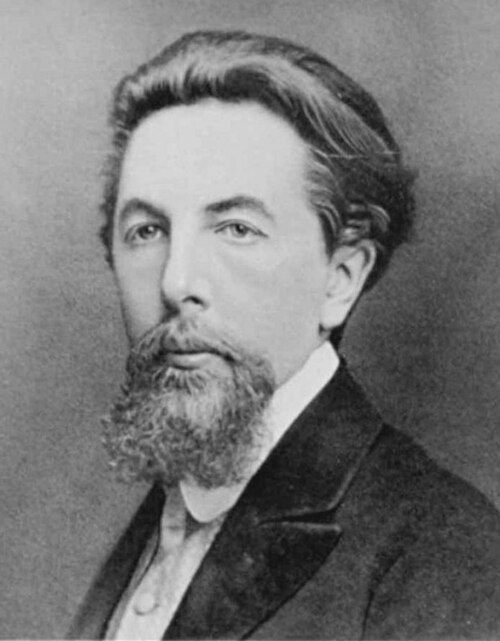
\includegraphics[width=\linewidth]{images/book3/tsvet.jpg}
\end{minipage}\hfill
\begin{minipage}[t]{0.78\linewidth}
\vspace{0pt}
植物学家米哈伊尔·茨维特将绿叶提取液倒入装有粉状
白垩的玻璃管中，再用溶剂淋洗，色素便分成有色谱带：绿色的
叶绿素和黄色的类胡萝卜素。1906 年，他将这一方法命名为色谱法（“颜色书写”）。
此后约四分之一个世纪里几乎无人问津，直到
1930 年代才被重新用于天然产物研究。（肖像：作者不详，公有领域；维基共享资源。）
\end{minipage}
\end{history}

\begin{safety}{\ghs[5mm]{GHS02}\,\ghs[5mm]{GHS05}\,\ghs[5mm]{GHS06}\,\ghs[5mm]{GHS07}\,\ghs[5mm]{GHS08}\,\ghs[5mm]{GHS09}}
乙腈和甲醇是 HPLC 流动相中常用的有机组分，二者易燃且有毒；
己烷用于柱色谱，易燃，有健康危害，并对水生生物有毒。
溶剂废液须单独收集，切勿倒入水槽。
% ledger: ghs:acetonitrile, ghs:methanol, ghs:hexane
\end{safety}

\section{练习}

\begin{exercise}[$\star$]\label{exo:b2:chromatography:1}
某化合物在死时间为 \qty{1.0}{min} 的色谱柱上，保留时间 $t_R = \qty{5.0}{min}$。
计算其保留因子，以及它在流动相中所占时间的分数。
\end{exercise}

\begin{exercise}[$\star$]\label{exo:b2:chromatography:2}
某峰在 $t_R = \qty{6.0}{min}$ 处出峰，基线宽度为 \qty{0.30}{min}。计算理论塔板数。
\end{exercise}

\begin{exercise}[$\star$]\label{exo:b2:chromatography:3}
在 \qty{250}{mm} 的色谱柱上，某化合物得到 $N = 10\,000$。计算理论塔板高度。
\end{exercise}

\begin{exercise}[$\star$]\label{exo:b2:chromatography:4}
判断下列分析应选用气相色谱还是高效液相色谱：血液中的乙醇；蛋白质；饮料中的咖啡因；汽油中的苯；果汁中的糖。
\end{exercise}

\begin{exercise}[$\star\star$]\label{exo:b2:chromatography:5}
两峰：$t_{R1} = \qty{4.0}{min}$，$w_1 = \qty{0.40}{min}$；$t_{R2} = \qty{4.6}{min}$，$w_2 =
\qty{0.50}{min}$。计算分离度，并判断两峰是否基线分离。
\end{exercise}

\begin{exercise}[$\star\star$]\label{exo:b2:chromatography:6}
两种化合物的选择因子 $\alpha = 1.10$，$k_2 = 4.0$，要使分离度达到
$R_s = 1.5$，需要多少块理论塔板？
\end{exercise}

\begin{exercise}[$\star\star$]\label{exo:b2:chromatography:7}
某色谱柱的参数为 $A = \qty{5}{\micro m}$，$B = \qty{8}{\micro m.mm/s}$，$C = \qty{2}{\micro m.s/mm}$
（练习数据）。求最佳流速和最小理论塔板高度。
\end{exercise}

\begin{exercise}[$\star\star$]\label{exo:b2:chromatography:8}
在反相 HPLC 中预测苯、苯酚和甲苯的洗脱顺序，所用流动相为
水–甲醇，并说明提高甲醇比例时会发生什么。
\end{exercise}

\begin{exercise}[$\star\star$]\label{exo:b2:chromatography:9}
一份待测物浓度为 \qty{20.0}{mg/L}、内标浓度为 \qty{10.0}{mg/L} 的校准溶液，
得到峰面积 860 和 400。向样品中加入 \qty{10.0}{mg/L} 的内标，得到峰面积 645 和 410。
计算响应因子和待测物的浓度（练习数据）。
\end{exercise}

\begin{exercise}[$\star\star\star$]\label{exo:b2:chromatography:10}
某次分离的 $R_s = 1.06$。相对于现用色谱柱，柱长需为多少才能使 $R_s = 1.5$，
这会多花多少时间？还有哪些其他的杠杆？
\end{exercise}

\begin{exercise}[$\star\star\star$]\label{exo:b2:chromatography:11}
对两个等高、等宽、基线宽度为 $w = 4\sigma$ 的高斯峰，计算两峰中点处的信号，
相对于峰高的值，分别在 $R_s = 1$ 和 $R_s = 1.5$ 时求出（忽略远峰在
每个极大值处的贡献）。
\end{exercise}

\begin{exercise}[$\star\star\star$]\label{exo:b2:chromatography:12}
在 $N$ 与 $\alpha$ 不变的条件下，比较分离度因子 $k_2/(1+k_2)$ 与相对分析时间
$1 + k_2$，分别取 $k_2 = 2$、5 和 10。应选哪一段 $k$ 范围？
\end{exercise}

\section{问题：能量饮料中的咖啡因}

\begin{problem}[{周末问题——反相洗脱顺序，由色谱图评价柱效，改善分离，以及
用内标法定量}]
\label{pb:b2:chromatography:1}
练习数据（虚构，并非真实方法）。将能量饮料稀释十倍（由 \qty{5.00}{mL} 稀释至
\qty{50.0}{mL}），并在稀释液中加入茶碱作内标，浓度为 \qty{40.0}{mg/L}。
溶液。色谱柱规格为 \qty{150}{mm}，反相色谱；流动相为水–甲醇，采用紫外检测。未被保留的
基质（糖类和盐）在 $t_M = \qty{1.0}{min}$ 处流出；茶碱在
\qty{3.0}{min} 处出峰（基线宽度 \qty{0.18}{min}）；咖啡因在 \qty{3.4}{min} 处出峰（基线宽度 \qty{0.20}{min}）。
校准：咖啡因 \qty{50.0}{mg/L} 与茶碱 \qty{40.0}{mg/L} 的峰面积分别为 1500 和 1000。
样品：峰面积 970（咖啡因）和 1010（茶碱）。每罐容量为 \qty{250}{mL}。
% ledger: ghs:caffeine, ghs:methanol

\begin{center}
\begin{tikzpicture}
\begin{axis}[width=0.75\linewidth, height=4.4cm, xmin=0, xmax=5, ymin=0, ymax=1,
  xlabel={时间 (min)}, ylabel={吸光度 (a.u.)}, label style={font=\small},
  tick label style={font=\scriptsize}, ytick=\empty]
\addplot[omDef, thick] table[x=t, y=s] {figdata/out/bachelor-2-chromatogram-c.dat};
\node[font=\scriptsize] at (axis cs:1.0,0.42) {基质};
\node[font=\scriptsize] at (axis cs:2.62,0.86) {茶碱};
\node[font=\scriptsize] at (axis cs:3.85,0.84) {咖啡因};
\end{axis}
\end{tikzpicture}
\end{center}
% figdata: bachelor-2/chromatogram.py part c

\medskip
\noindent\textbf{第一部分——反相。}
\begin{enumerate}
  \item 描述反相色谱柱的固定相和流动相。
  \item 为什么糖类在死时间洗脱出来？
  \item 咖啡因是 1,3,7-三甲基黄嘌呤，茶碱是 1,3-二甲基黄嘌呤。
        解释它们的洗脱顺序。
  \item 为什么茶碱在这里是一个良好的内标？
  \item 若提高甲醇的比例，两个保留时间会发生什么变化？
  \item 死时间测量的是什么？
\end{enumerate}

\medskip
\noindent\textbf{第二部分——柱效。}
\begin{enumerate}[resume]
  \item 计算茶碱和咖啡因的比移值。
  \item 计算选择因子。
  \item 分别计算咖啡因和茶碱的理论塔板数。
  \item 计算咖啡因的理论塔板高度。
  \item 计算两个峰之间的分离度。
  \item 用分离度方程进行验算。
  \item 两个峰是否完全分离（基线分离）？
\end{enumerate}

\medskip
\noindent\textbf{第三部分——更快还是更好？}
\begin{enumerate}[resume]
  \item 为节省时间，将色谱柱缩短至 \qty{75}{mm}（填料和流速不变）。
        分离度会怎样变化？
  \item 分析时间又会怎样？
  \item 改用 \qty{300}{mm} 的色谱柱会得到什么结果？付出什么代价？
  \item 哪一个杠杆作用于 $\alpha$？
  \item 在这里提高 $k$ 会有较大帮助吗？
\end{enumerate}

\medskip
\noindent\textbf{第四部分——定量分析。}
\begin{enumerate}[resume]
  \item 计算咖啡因相对于茶碱的响应因子。
  \item 为什么进样体积无关紧要？
  \item 计算稀释后溶液中咖啡因的浓度。
  \item 计算饮料中咖啡因的浓度。
  \item 若某基质化合物与茶碱共洗脱，会出现什么问题？
  \item 外标法需要什么？
  \item 求一罐 \qty{250}{mL} 饮料罐中咖啡因的质量。
\end{enumerate}
\end{problem}
